\documentclass[border=3pt]{standalone}
% Preâmbulo compartilhado pelos diagramas TikZ da aula 5 de IHC (Processos de Design)
\usepackage[T1]{fontenc}
\usepackage[utf8]{inputenc}
\usepackage{lmodern}
\usepackage{amsmath}
\usepackage{xcolor}
\usepackage{tikz}
\usetikzlibrary{arrows.meta,angles,quotes,decorations.pathmorphing,calc,
                positioning,shapes.geometric,shapes.misc,backgrounds,fit,
                math}

% Paleta (mesma dos SVGs originais)
% Paleta da disciplina de IHC: acento roxo (#755099), da capa do livro.
% (o nome "dblue" é mantido para não alterar todos os diagramas)
\definecolor{dblue}{HTML}{755099}
\definecolor{dorange}{HTML}{B3541E}
\definecolor{dgreen}{HTML}{4A7C59}
\definecolor{dred}{HTML}{9C4B4B}
\definecolor{dcream}{HTML}{F4F1EA}
\definecolor{dshade}{HTML}{DDD7C9}

% Função gaussiana (não normalizada por padrão de escala visual)
\pgfmathdeclarefunction{gauss}{3}{%
  \pgfmathparse{1/(#3*sqrt(2*pi))*exp(-((#1-#2)^2)/(2*#3^2))}%
}

% Estilos comuns (prefixo d... para não colidir com chaves internas do pgf)
\tikzset{
  >={Stealth[length=2mm]},
  dguide/.style={gray!55, dashed, line width=0.4pt},
  daxis/.style={gray!60, line width=0.7pt, ->},
  dbody/.style={fill=black!3, draw=black!80, line width=1pt},
  dacc/.style={draw=dblue, line width=1pt},
  dlbl/.style={black!55, font=\small},
  dsub/.style={black!45, font=\footnotesize},
  dstate/.style={circle, draw=black!80, fill=dcream, line width=1pt,
                 minimum size=17mm, font=\large, inner sep=1pt},
  dobs/.style={circle, draw=black!80, fill=dshade, line width=1pt,
               minimum size=14mm, font=\large, inner sep=1pt},
  dbox/.style={rounded corners=2pt, draw=black!80, fill=dcream, line width=1pt,
               align=center, inner sep=6pt},
  dop/.style={circle, draw=black!80, fill=white, line width=1pt,
              minimum size=6mm, inner sep=0pt, font=\small},
  dtrans/.style={->, dblue, line width=1pt},
  dmeas/.style={->, dorange, line width=1pt},
  dcurve/.style={line width=1pt, dblue},
  dcurveb/.style={line width=1.4pt, dorange},
}

\begin{document}
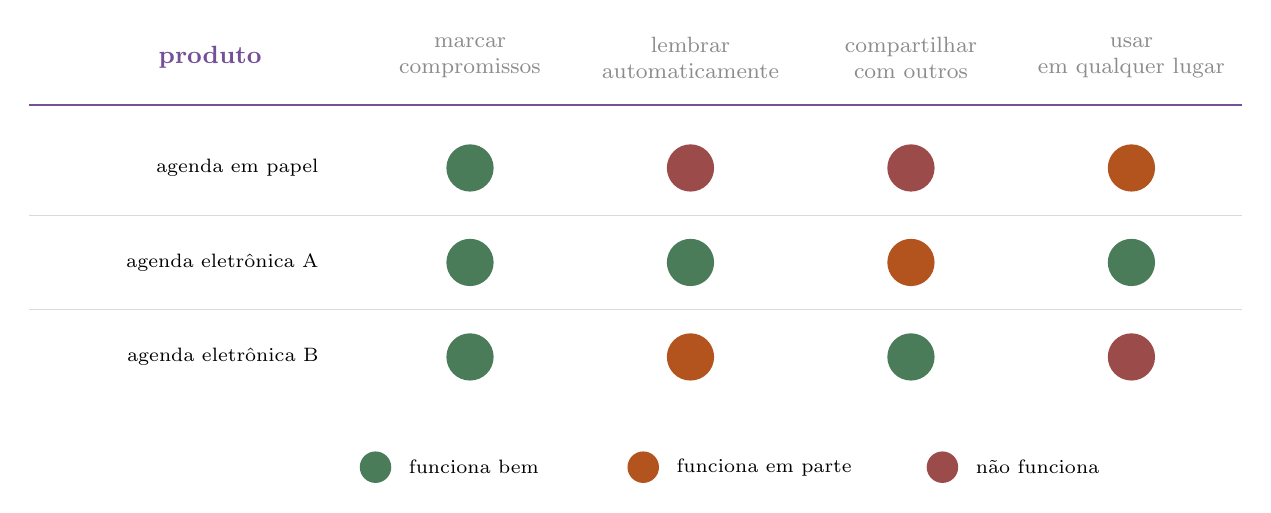
\begin{tikzpicture}[x=1cm,y=1cm]

  \newcommand{\ok}[2]{\fill[dgreen] (#1,#2) circle (0.3);}
  \newcommand{\parc}[2]{\fill[dorange] (#1,#2) circle (0.3);}
  \newcommand{\nao}[2]{\fill[dred] (#1,#2) circle (0.3);}

  \node[font=\small\bfseries, dblue] at (1.9,3.3) {produto};
  \foreach \x/\t in {5.2/{marcar\\compromissos},8.0/{lembrar\\automaticamente},10.8/{compartilhar\\com outros},13.6/{usar\\em qualquer lugar}} {
    \node[font=\scriptsize, align=center, dsub] at (\x,3.3) {\t};
  }
  \draw[dblue, line width=1pt] (-0.4,2.7) -- (15.0,2.7);

  \node[anchor=east, font=\scriptsize] at (3.4,1.9) {agenda em papel};
  \ok{5.2}{1.9} \nao{8.0}{1.9} \nao{10.8}{1.9} \parc{13.6}{1.9}
  \node[anchor=east, font=\scriptsize] at (3.4,0.7) {agenda eletrônica A};
  \ok{5.2}{0.7} \ok{8.0}{0.7} \parc{10.8}{0.7} \ok{13.6}{0.7}
  \node[anchor=east, font=\scriptsize] at (3.4,-0.5) {agenda eletrônica B};
  \ok{5.2}{-0.5} \parc{8.0}{-0.5} \ok{10.8}{-0.5} \nao{13.6}{-0.5}
  \foreach \y in {1.3,0.1} { \draw[black!15, line width=0.5pt] (-0.4,\y) -- (15.0,\y); }

  \fill[dgreen] (4.0,-1.9) circle (0.2); \node[anchor=west, font=\scriptsize] at (4.3,-1.9) {funciona bem};
  \fill[dorange] (7.4,-1.9) circle (0.2); \node[anchor=west, font=\scriptsize] at (7.7,-1.9) {funciona em parte};
  \fill[dred] (11.2,-1.9) circle (0.2); \node[anchor=west, font=\scriptsize] at (11.5,-1.9) {não funciona};


\end{tikzpicture}
\end{document}
